\documentclass[a4paper,12pt]{article}
\usepackage[utf8]{inputenc}
\usepackage{tikz}
\usepackage{amsmath, amssymb, amsthm} % for mathematical symbols
\usepackage{geometry} % for setting page dimensions
\usepackage{datetime}

% Define a new theorem-like environment for Examples
\newtheoremstyle{example}
  {3pt} % Space above
  {3pt} % Space below
  {\itshape} % Body font
  {} % Indent amount
  {\bfseries} % Theorem head font
  {.} % Punctuation after theorem head
  {.5em} % Space after theorem head
  {} % Theorem head spec (can be left empty, meaning `normal`)

\theoremstyle{example}
\newtheorem{example}{Example}[section]


\theoremstyle{definition}
\newtheorem{definition}{Definition}[section]

\theoremstyle{remark}
\newtheorem*{remark}{Remark}

\newtheorem{theorem}{Theorem}[section]
\newtheorem{corollary}{Corollary}[theorem]
\newtheorem{lemma}[theorem]{Lemma}


\newdate{date}{28}{08}{2024}
\date{\displaydate{date}}
\geometry{margin=1in}

\begin{document}

% Lecture note scribed by Ethan Hong

% First page header information
\begin{center}
    \Large \textbf{CSE 540 Wk1} \\ % Course name
    \vspace{0.5cm}
    \large \displaydate{date}
    \vspace{0.5cm}
\end{center}

In the last lecture we visited the motivation behind complexity theory. In this lecture we will introduce the basic idea and intuition for Turing machines.

\subsection{Why Turing machines}

In the undergraduate level computation class, we may have already studied multiple computation models including Finite State Machines (FSMs), Push Down Automatas (PDAs), and maybe some introductions on Turing machines. A natrual question to ask even before studying the Turing machine is: Why is Turing machine needed? And what tasks we can perform with a turing machine but not with a FSM or PDA?



\begin{figure}[h]
    \centering
    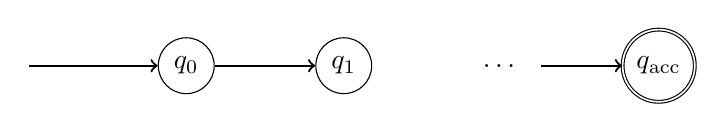
\begin{tikzpicture}
        % Draw the states in a horizontal line
        \node[draw, circle, minimum size=0.5cm, align=center] (q1) at (-2, 0) {$q_0$};
        \node[draw, circle, minimum size=0.5cm, align=center] (q2) at (0, 0) {$q_1$};
        
        % Ellipsis ("...")
        \node at (2, 0) {\dots};
    
        % Accepting state with double circle
        \node[draw, double, circle, minimum size=0.5cm, align=center] (qacc) at (4, 0) {$q_{\text{acc}}$};
    
        % Arrows
        \draw[->, thick] (-4, 0) -- (q1); % Arrow pointing to q1
        \draw[->, thick] (q1) -- (q2); % Arrow from q1 to q2
        \draw[->, thick] (2.5, 0) -- (qacc); % Arrow from "..." to q_acc
    \end{tikzpicture}
    \caption{A Finite State Machine}
    \label{fig:fsm}
\end{figure}

The intuition is, with FSMs, we can do certain computations, maybe decide a regular language. But it can not do much more than that (for example, it won't be able to recognize the language $\left\{0^k1^k \mid k \in \mathbb{N} \right\}$).

So people came up with another model, adding a stack to the finite state machine, but it has its limitations (for example, it won't be able to recognize the language $\left\{0^k1^k0^k \mid k \in \mathbb{N}\right\}$)

Both Finite State Machines and Push Down Automatas has certain capability, and some "built-in" memory (states, stack), however their memory is limited. For example, finite state machines can not "remember" how many 0's it has seen and match that with the following 1's, and similarly even if we give it a stack it can only sort of memorize one thing at a time. Thus, we now introduce a machine that can memorize ...

\subsection{Introduction to Turing Machines}
Imagine the tape of a cassette, for Finite Automatas, the input goes one-way. For example, given $(000111) \in \left\{0,1\right\}^{*}$, and a finite automata $F$, after reading the first 3 zeros, it can't not go back and read the zeros again. On the other hand, in a turing machines, we give it the power, letting the head pointer for the input tape to move freely so that it could read the zeros again.

\begin{definition}[Turing Machine (informal)]
A Turing Machine M 
\end{definition}
\subsection{A few examples regarding Turing Machines}


\begin{example}[Erase]
Given an input $x \in \left\{0,1\right\}^{*}$ , erase the input (i.e. replace the input with blank character).
\end{example}



\begin{example}[Copy]
Given an input $x \in \left\{0,1\right\}^{*}$, copy the input string to the end.
\end{example}


\begin{example}[Addition]

\end{example}

\begin{example}[Sorting]
\end{example}
\subsection{Why tape size doesn't matter, and Oblivious Turing Machines}

\end{document}
